% !TEX root = NSF_SuperCDMS_SNOLAB_OPS.tex
%% people who build community and knowledge
%% around software?
%% The maintainers
%% Educopia
%% http://ivory.idyll.org/blog/2019-communities-of-effort.html#disqus_thread
%% https://blog.dnanexus.com/2018-01-29-analysis-commons-a-collaborative-approach-to-multi-omics-discovery/

%% describing data
%https://library.si.edu/research/describing-your-data-data-dictionaries
%https://figshare.com/articles/The_State_of_Open_Data_Report_2017/5481187/1
%https://www.usgs.gov/products/data-and-tools/data-management/data-standards
%https://www.fgdc.gov/standards/standards_publications/
%http://www.ddialliance.org/ metadata standards for social sciences
%https://www.rd-alliance.org/groups/data-type-registries-wg.html research data alliance, not focused on physics AFAIK but definitely useful
%https://access-data.trydiscourse.com/

% Mom says all the cool kids are using smartsheets
% Liquid Planner has a free plan for teachers?  https://app.liquidplanner.com/space/202855/projects


\subsection{Introduction}

\subsection{Science-driven}
% How will the project outcomes fill well-recognized science and engineering needs of the research community, and advance research capability within a significant area or areas of science and engineering? What are the broader impacts of the project, such as benefits to science and engineering communities beyond initial targets, underrepresented communities, and education and workforce development? The project outcomes should address well-recognized science outcomes.

This project serves the immediate needs of researchers in the dark matter community and the experimental nuclear physics community by providing a common toolset for analyzing data in any format.

The PI expects that

\begin{itemize}
    \item Multiple research projects across the NSF directorate will be more productive because they can use existing, documented tools rather than building their own.  The PI intends to estimate this impact with citations from scientific papers.
    \item Increased involvement of undergraduate researchers in science analysis due to improved documentation and an extended support network.  The PI intends to measure this through undergraduate involvement in her own lab, community surveys, and tracking community forum data.
    \item Several example analyses will be publicly released, with accompanying documentation and support information for pre-requisite computing skills.  The intent is for these educational materials to be accessible to someone with no domain knowledge.  The PI believes these training materials will be an equitable training resource.
\end{itemize}


\subsection{Innovation}
% What innovative and transformational capabilities will the project bring to its target communities, and how will the project integrate innovation and discovery into the project activities, such as through empirical research embedded as an integral component of the project activities? Such research might encompass reproducibility, provenance, effectiveness, usability, and adoption of the components, adaptability to new technologies and to changing requirements, and the development of lifecycle processes used in the project.

A common limitation of data-analysis software that is entirely home-grown is that it does not scale as data grows and changes - a human has to update or rewrite the code if the requirements change substantially.

This library makes heavy use of existing libraries.  The benefit is that as those libraries improve and scale to larger data sets, this software inherits that improvement.  

In both cases, significant human effort is needed to adapt the software to changing data and needs.  But by leveraging well-supported, open-source libraries, the burden is shifted away from an individual scientist and towards an active community that is highly motivated to solve similar problems.  This library serves as sugar to allow scientists with many different data formats to take advantage of these popular libraries.

The danger to this approach is the same - if these libraries lose community support or focus on very different problems then this library will lose relevance over time.  To mitigate this risk, the PI is focusing on integrating with a library supported by the IRIS-HEP collaboration and with pandas, which enjoys extreme popularity in the data science community.

\subsection{Close collaboration among stakeholders}
% How will the project activities engage CI experts, specialists, and scientists and engineers working in concert with the relevant domain scientists and engineers who are users of CI?

The PI proposes to engage both cyberinfrastructure experts and the experimental nuclear physics community by (1) working closely with pilot experiments to build software that works effectively for scientists analyzing event-based data, (2) holding yearly workshops intended to foster interaction between the scientists using the software and cyberinfrastructure developers, and (3) attending conferences that will allow outreach to the scientific community (for example, the Low Energy Community Meeting) and the cyberinfrastructure community (for example, CHEP).

The PI has working relationships with scientists in the SuperCDMS collaboration and the XIA corporation, both of which are interested in exploring the proposed software as solutions to analysis needs.

In addition, the IRIS-HEP collaboration is interested in this work as it would extend their awkward-array library to a broader audience.  Awkward array was developed by Jim as part of DIANA/HEP (http://diana-hep.org,
OAC-1450377) and that effort will continue with IRIS-HEP
(http://iris-hep.org, OAC-1836650).  Collaborating with IRIS-HEP gives us access to experienced cyberinfrastructure developers who have focused on developing software suitable for terabyte-scale data.


\subsection{Building on existing, recognized capabilities}
% How will the project activities build on and leverage existing NSF and national cyberinfrastructure investments, as appropriate?

The proposed work builds on existing capabilities and communities in several ways:

\begin{itemize}
    \item \textbf{The PI proposes to use already-existing data description languages.}  The languages Katai Struct and the Data Format Description Langauage both have active communities and tools that work with data when provided a description.  Kaitai Struct is the target for the proposed work because (1) it is more human-readable than than the XML-based DFDL, and (2) Katai Struct generates code libraries that allow users to load their data into the programming environment of their choice; DFDL currently works by providing an XML or JSON equivalent of the binary data.  While this is a powerful approach because any language with an XML or JSON parser can now read the data, it also produces a secondary data file that is an order of magnitude larger than most binary files.  This makes DFDL, in its current state, unusable for scientists with gigabyte-scale data sets as it would make the required storage space for analysis prohibitively expensive.
    \item \textbf{The PI proposes to use already-existing infrastructure for the data-analysis library.}  Scientists who would like to avoid writing custom software to read their binary data can already use the Kaitai Struct compiler to generate libraries to read their data in python, C++, and a multitude of other languages.  The advantage is that there is substantial support documentation and an active community available for troubleshooting.  The disadvantage is that the current Kaitai Struct python compiler stores the data in a structure that does not provide adequate speed performance for gigabyte-scale data sets.  By improving the existing Katai Struct compiler software, we can build a science-ready analysis library and scientists can benefit from the existing community support and documentation.   
    \item \textbf{Use a supported and optimized data structure}  for the improvements to the Kaitai Struct compiler.  The ``awkward-array'' library was developed by DIANA/HEP and is now supported by IRIS-HEP and is part of a set of libraries designed to provide flexible data-analysis tools for the high-energy physics community.  The awkward-array data structure is optimized for fast queries on an event-based data set and as such is ideal for the majority of nuclear physics data.  By choosing this data structure as the target, we bring the optimized and convenient analysis environment of awkward-array to any scientist who describes their data with the Katai Struct language.
    \item \textbf{Provide analysis tools for the python environment and training materials that take advantage of the python ecosystem.}  Python is a popular analysis environment in the field of big-data and has enjoyed significant adoption in the scientific community; enough so that python support is compiled in the dominant high-energy physics software, ROOT, by default.  By providing a python library for data analysis, scientists can make use of a full ecosystem that supports data analysis: numpy for convenient array manipulation; scipy for fitting; matplotlib for producing publication-quality figures; and even numba for easy compilation of code that needs to run fast.  This entire environment is easily installed - even for users without administration privileges - through the Anaconda Python distribution.  There are many free and paid programming environments that are availble, notably the Jupyter environment.  Code written in this environment is particularly nice as a tutorial because it is rendered nicely on github, gitlab, and interactive notebooks can be opened in one click through binder.  By providing a small set of introductory documentation, scientists can benefit from the effort the python community has put in to lower the barrier for use.
    
\end{itemize}

\subsection{Project plans, and system and process architecture}
% For an "Elements" proposal, the Project Description should include a high-quality management plan. The proposal should include user interactions and a community-driven approach, and provide a timeline including a proof-of-concept demonstration of the key components. Software or data cyberinfrastructure services should be sufficiently described and follow industry best practices, including the architecture of the CI and the engineering process to be used for the design, development, documentation, testing, validation, and release of the software, its deployment and associated outreach to the end user community, and an acceptance and evaluation plan that involves end users. The description of the CI architecture and processes should explain how security, trustworthiness, provenance, reproducibility, and usability will be addressed by the project and integrated into the proposed system and the engineering process, and how adaptability to new technologies and changing requirements will be addressed by the project and built into the proposed system, as appropriate.

The timing of the proposed work is driven by the proposed, yearly workshops that focus on (1) teaching scientists how to use the tools to access their data, (2) working with scientists to perform their analyses in the python environment, (3) identifying improvements needed for the software to be easy to learn and useful in analysis, and (4) bringing developers into close contact with the science community using their tools.  Each workshop will result in an updated roadmap for the software.

Thus, the workshops - and software releases that include testing, documentation, and example analyses - are the primary milestones of the proposed work.

The work for each yearly cycle can be broken down into the following categories:


\begin{figure}[htb]
    \begin{center}
      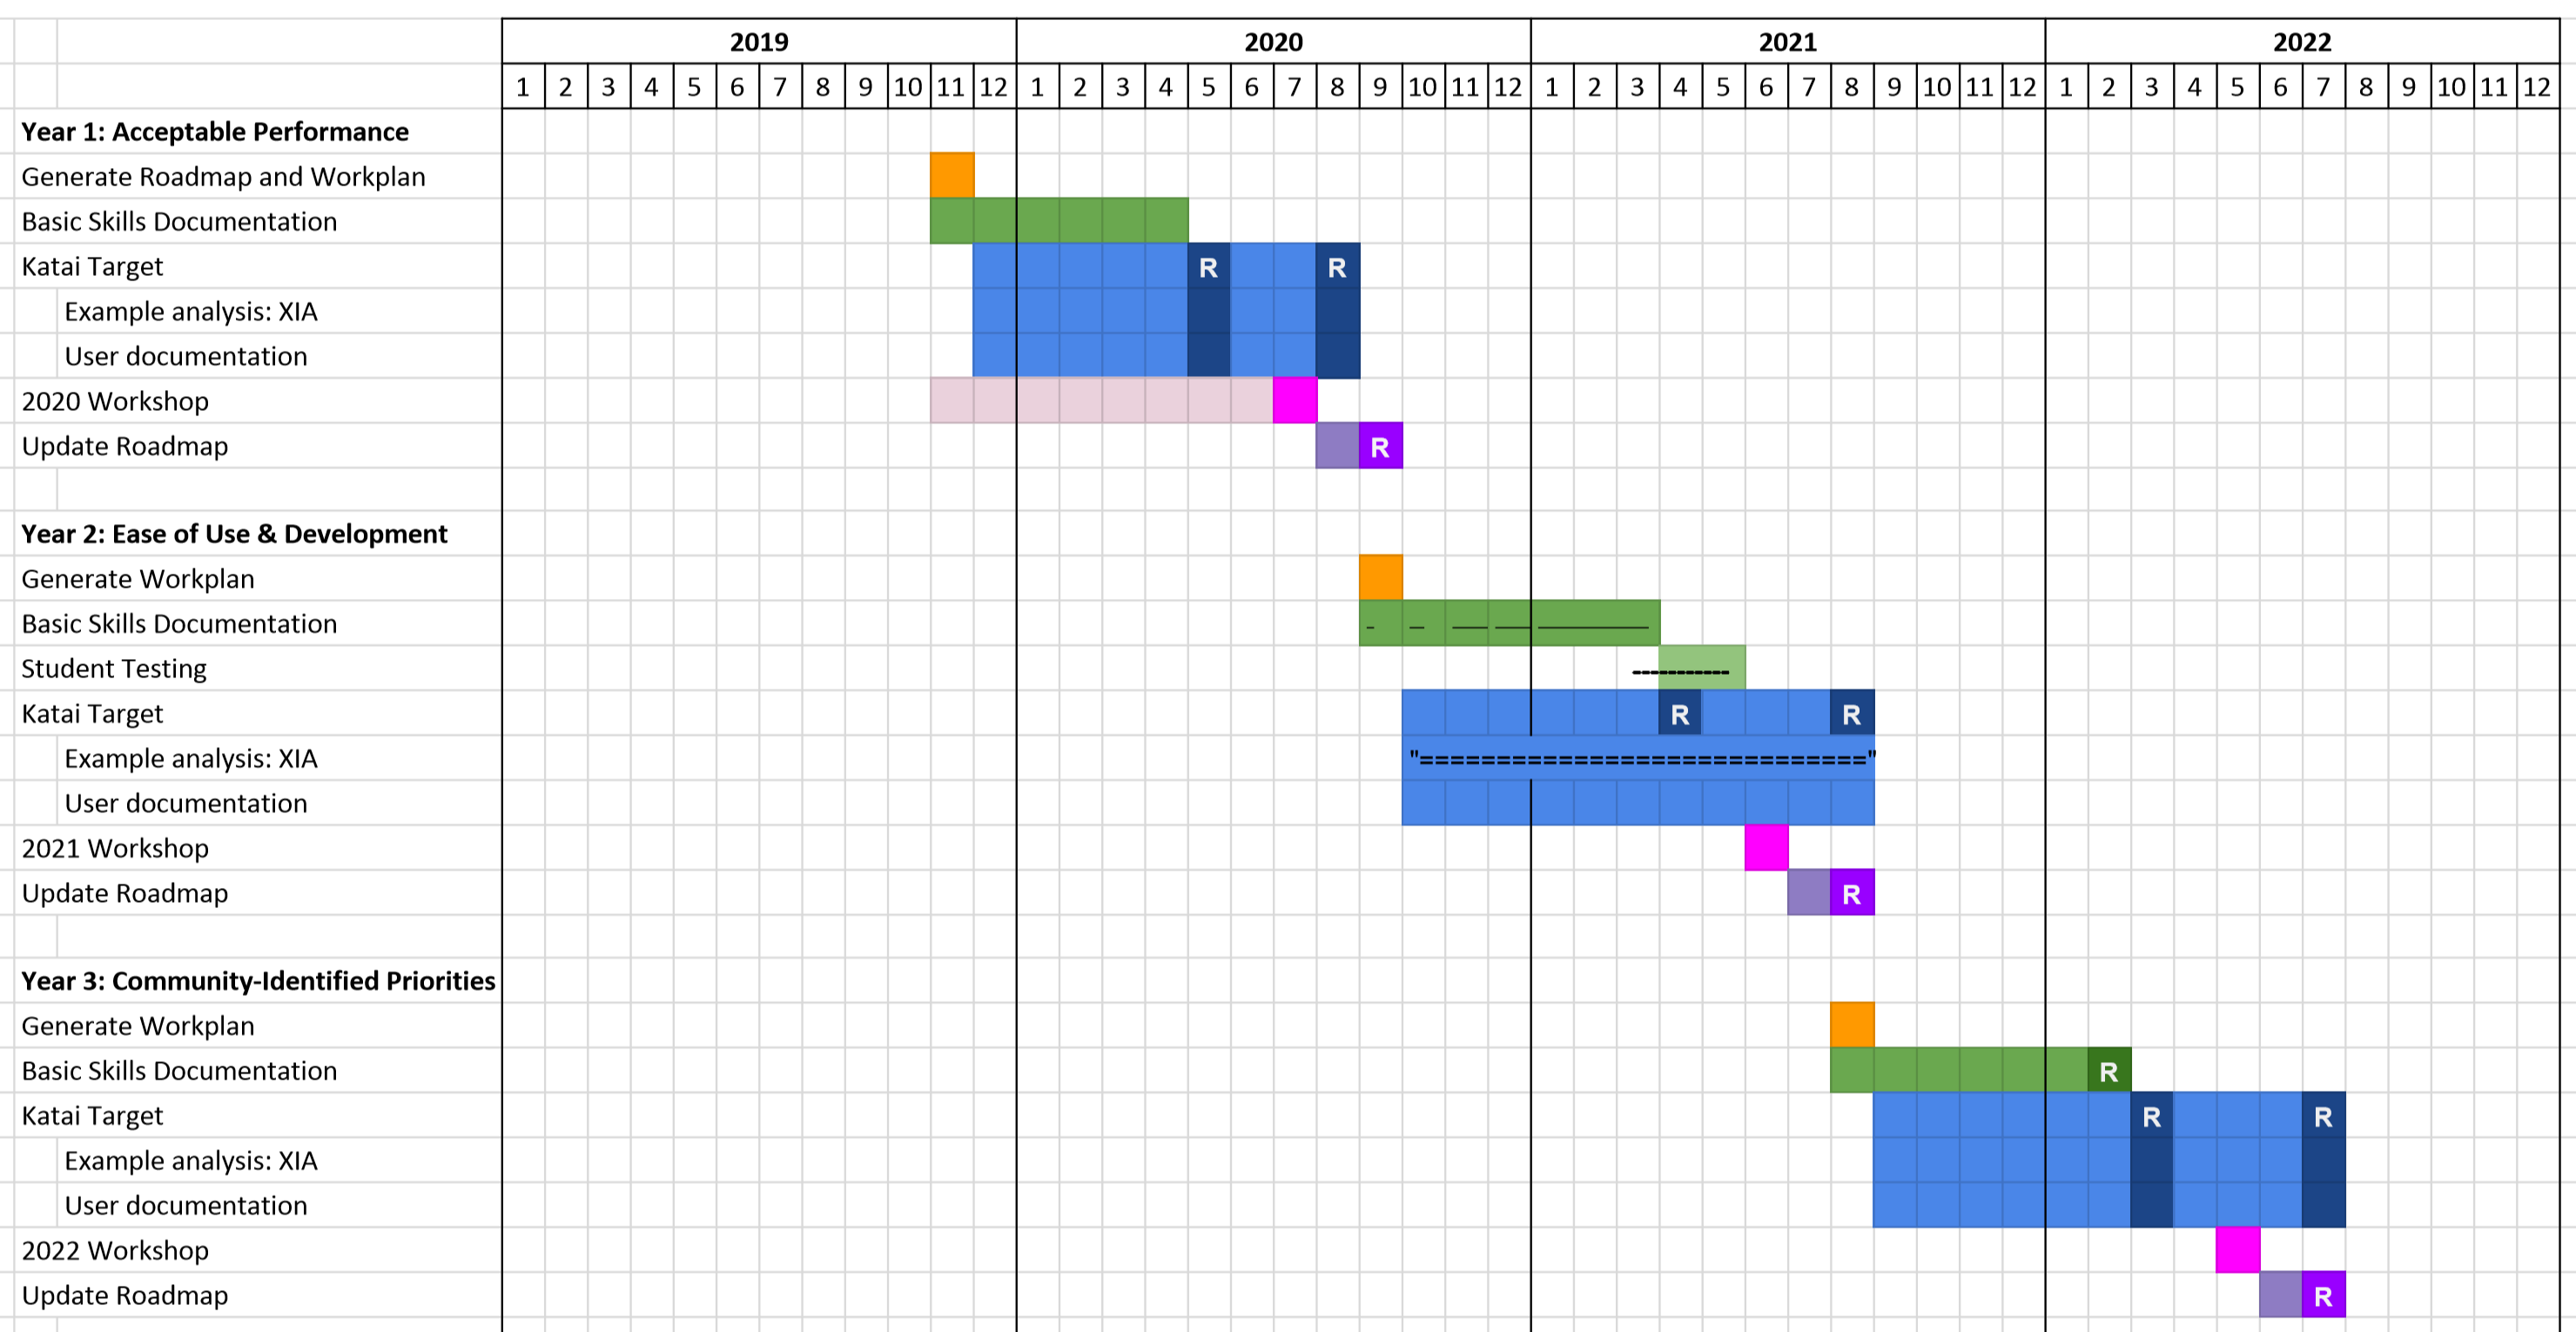
\includegraphics[width=\textwidth]{Figures/schedule1}
    \end{center}
    \caption{Schedule for the \scs Experiment.}
    \label{fig:ops-schedule}
\end{figure}

\subsection{Deliverables}


\subsection{Metrics}


\subsection{Sustained and sustainable impacts}